%%%%%%%%%%%%%%%%%%%%%%%%%%%%%%%%%%%%%%%%%
% Masters/Doctoral Thesis 
% LaTeX Template
% Version 1.43 (17/5/14)
%
% This template has been downloaded from:
% http://www.LaTeXTemplates.com
%
% Original authors:
% Steven Gunn 
% http://users.ecs.soton.ac.uk/srg/softwaretools/document/templates/
% and
% Sunil Patel
% http://www.sunilpatel.co.uk/thesis-template/
%
% License:
% CC BY-NC-SA 3.0 (http://creativecommons.org/licenses/by-nc-sa/3.0/)
%
% Note:
% Make sure to edit document variables in the Thesis.cls file
%
%%%%%%%%%%%%%%%%%%%%%%%%%%%%%%%%%%%%%%%%%

%----------------------------------------------------------------------------------------
%	PACKAGES AND OTHER DOCUMENT CONFIGURATIONS
%----------------------------------------------------------------------------------------

\documentclass[13pt, oneside]{Thesis} % The default font size and one-sided printing (no margin offsets)

\graphicspath{{Pictures/}} % Specifies the directory where pictures are stored

\usepackage[square, numbers, comma, sort&compress]{natbib} % 

\usepackage{listings}
\usepackage{color}
\usepackage{mathtools}

\definecolor{dkgreen}{rgb}{0,0.6,0}
\definecolor{gray}{rgb}{0.5,0.5,0.5}
\definecolor{mauve}{rgb}{0.58,0,0.82}

\lstdefinelanguage{scala}{
  morekeywords={abstract,case,catch,class,def,%
    do,else,extends,false,final,finally,%
    for,if,implicit,import,match,mixin,%
    new,null,object,override,package,%
    private,protected,requires,return,sealed,%
    super,this,throw,trait,true,try,%
    type,val,var,while,with,yield},
  otherkeywords={=>,<-,<\%,<:,>:,\#,@},
  sensitive=true,
  morecomment=[l]{//},
  morecomment=[n]{/*}{*/},
  morestring=[b]",
  morestring=[b]',
  morestring=[b]"""
}

\hypersetup{urlcolor=blue, colorlinks=true} % Colors hyperlinks in blue - change to black if annoying
\title{\ttitle} % Defines the thesis title - don't touch this

\begin{document}

\frontmatter % Use roman page numbering style (i, ii, iii, iv...) for the pre-content pages

\setstretch{1.3} % Line spacing of 1.3

% Define the page headers using the FancyHdr package and set up for one-sided printing
\fancyhead{} % Clears all page headers and footers
\rhead{\thepage} % Sets the right side header to show the page number
\lhead{} % Clears the left side page header

\pagestyle{fancy} % Finally, use the "fancy" page style to implement the FancyHdr headers

\newcommand{\HRule}{\rule{\linewidth}{0.5mm}} % New command to make the lines in the title page

% PDF meta-data
\hypersetup{pdftitle={\ttitle}}
\hypersetup{pdfsubject=\subjectname}
\hypersetup{pdfauthor=\authornames}
\hypersetup{pdfkeywords=\keywordnames}

%----------------------------------------------------------------------------------------
%	TITLE PAGE
%----------------------------------------------------------------------------------------

\begin{titlepage}
\begin{center}

\textsc{\LARGE \univname}\\[1.5cm] % University name
\textsc{\Large Master Thesis}\\[0.5cm] % Thesis type

\HRule \\[0.4cm] % Horizontal line
{\huge \bfseries \ttitle}\\[0.4cm] % Thesis title
\HRule \\[1.5cm] % Horizontal line
 
\begin{minipage}{0.4\textwidth}
\begin{flushleft} \normalsize
\emph{Author:}\\
\href{hoang@eurecom.fr}{\authornames} % Author name - remove the \href bracket to remove the link
\end{flushleft}
\end{minipage}
\begin{minipage}{0.4\textwidth}
\begin{flushright} \normalsize
\emph{Supervisor:} \\
\href{michiard@eurecom.fr}{\supname} % Supervisor name - remove the \href bracket to remove the link  
\emph{Academic Supervisor:}\\
\href{michiard@eurecom.fr}{\supname}\\
\href{phan@eurecom.fr}{Duy-Hung PHAN}\\
\end{flushright}
\end{minipage}\\[3cm]
 
\large \textit{A thesis submitted in fulfilment of the requirements\\ for the degree of \degreename}\\[0.3cm] % University requirement text
\textit{in the}\\[0.4cm]
\groupname\\\deptname\\[2cm] % Research group name and department name
 
{\large \today}\\[4cm] % Date
%\includegraphics{Logo} % University/department logo - uncomment to place it
 
\vfill
\end{center}

\end{titlepage}

%----------------------------------------------------------------------------------------
%	DECLARATION PAGE
%	Your institution may give you a different text to place here
%----------------------------------------------------------------------------------------

\Declaration{

\addtocontents{toc}{\vspace{1em}} % Add a gap in the Contents, for aesthetics

I, \authornames, declare that this thesis titled, '\ttitle' and the work presented in it are my own. I confirm that:

\begin{itemize} 
\item[\tiny{$\blacksquare$}] This work was done wholly or mainly while in candidature for a research degree at Eurecom Institute.
\item[\tiny{$\blacksquare$}] Where any part of this thesis has previously been submitted for a degree or any other qualification at this Institute or any other institution, this has been clearly stated.
\item[\tiny{$\blacksquare$}] Where I have consulted the published work of others, this is always clearly attributed.
\item[\tiny{$\blacksquare$}] Where I have quoted from the work of others, the source is always given. With the exception of such quotations, this thesis is entirely my own work.
\item[\tiny{$\blacksquare$}] I have acknowledged all main sources of help.
\item[\tiny{$\blacksquare$}] Where the thesis is based on work done by myself jointly with others, I have made clear exactly what was done by others and what I have contributed myself.\\
\end{itemize}
 
Signed:\\
\rule[1em]{25em}{0.5pt} % This prints a line for the signature
 
Date:\\
\rule[1em]{25em}{0.5pt} % This prints a line to write the date
}

\clearpage % Start a new page

%----------------------------------------------------------------------------------------
%	QUOTATION PAGE
%----------------------------------------------------------------------------------------

\pagestyle{empty} % No headers or footers for the following pages

\null\vfill % Add some space to move the quote down the page a bit


\vfill\vfill\vfill\vfill\vfill\vfill\null % Add some space at the bottom to position the quote just right

\clearpage % Start a new page

%----------------------------------------------------------------------------------------
%	ABSTRACT PAGE
%----------------------------------------------------------------------------------------

\addtotoc{Abstract} % Add the "Abstract" page entry to the Contents

\abstract{\addtocontents{toc}{\vspace{1em}} % Add a gap in the Contents, for aesthetics

Large-scale data analysis has grown enormously in recent years. For example, Hadoop MapReduce, the de-facto standard framework to process such huge amount of data, has undergone several evolutions, which materialized in a new framework called Apache Spark.\\
In large data warehouses, multiple queries can be submitted by users at the same time. In addition, it has been shown that different jobs can operate on the same input file (indeed, some data is “hotter” than other), so there is a high probability for sharing the cost of reading the input file and computation also.\\
In this project, we propose a framework that accepts multi-query workloads and proceeds with work-sharing optimization, for the Apache Spark system. In practice, we will focus on sharing I/O, the framework automatically detects and efficiently combine the sharable queries, which are combined into smaller number of jobs that will compute output for all shared queries. The framework also provides a scheduling mechanism which allows multi-query workloads to be optimized and executed in an efficient way.\\
}

\clearpage % Start a new page

%----------------------------------------------------------------------------------------
%	ACKNOWLEDGEMENTS
%----------------------------------------------------------------------------------------

\setstretch{1.3} % Reset the line-spacing to 1.3 for body text (if it has changed)

\acknowledgements{\addtocontents{toc}{\vspace{1em}} % Add a gap in the Contents, for aesthetics

I would like to express my special thanks of gratitude to Professeur Pietro MICHIARDI and Duy-Hung PHAN, who gave me the opportunity to do this project on the topic '\ttitle' and also gave me advises which helped me to accomplished the project.
}
\clearpage % Start a new page

%----------------------------------------------------------------------------------------
%	LIST OF CONTENTS/FIGURES/TABLES PAGES
%----------------------------------------------------------------------------------------

\pagestyle{fancy} % The page style headers have been "empty" all this time, now use the "fancy" headers as defined before to bring them back

\lhead{\emph{Contents}} % Set the left side page header to "Contents"
\tableofcontents % Write out the Table of Contents

\lhead{\emph{List of Figures}} % Set the left side page header to "List of Figures"
\listoffigures % Write out the List of Figures

\lhead{\emph{List of Tables}} % Set the left side page header to "List of Tables"
\listoftables % Write out the List of Tables

%----------------------------------------------------------------------------------------
%	THESIS CONTENT - CHAPTERS
%----------------------------------------------------------------------------------------

\mainmatter % Begin numeric (1,2,3...) page numbering

\pagestyle{fancy} % Return the page headers back to the "fancy" style

% Include the chapters of the thesis as separate files from the Chapters folder
% Uncomment the lines as you write the chapters

% Chapter 1

\chapter{Introduction} % Main chapter title

\label{Chapter1} % For referencing the chapter elsewhere, use \ref{Chapter1} 

\lhead{Chapter 1. \emph{Introduction}} % This is for the header on each page - perhaps a shortened title
Nowadays, large-scale data analysis has explosively grown. In the beginning of the big data era, Hadoop MapReduce \cite{hadoop} was the dominant framework which was widely used to process huge amount of data. Under several evolutions, a new framework appeared which is called Apache Spark \cite{spark}.

In general, writing a MapReduce \cite{Dean2004} algorithm in Hadoop and Spark requires exceptional skills, because of the intricacies of the underlying programming model: to overcome such problems, high-level languages (in essence, similar to SQL) have emerged as an alternative method to query data. For example, Apache Pig \cite{Gates2009} \cite{pig} and Apache Hive \cite{ashish2009} \cite{hive} bring to users the ability to express their programs in SQL-like by PigLatin \cite{Olston} and HiveQL \cite{ashish2009} , which are then compiled into MapReduce jobs before their execution. Apache Spark has also brought to us its SQL-like framework called SparkSQL \cite{michaelb}, which provides users the flexibilites of using Dataframe API and SQL.\\

In large data warehouses, multiple queries can be submitted by multiple users at the same time. Some files can be used at the input of many queries with different tasks. In other way, these files are "hotter" than the others because they are used more frequently, so they are high potential for sharing the cost of reading the input file and also the computations.\\

In this project, we propose a framework that accepts multi-query workloads and proceeds with work-sharing optimization, for the Apache Spark system. The framework automatically detects and efficiently combine the sharable queries, which are combined into smaller number of jobs that will compute output for all shared queries. The framework also provides a scheduling mechanism which allows multi-query workloads to be optimized and executed in an efficient way. The design of the framwork aims to provide users the generalization and extensibilities so many users can plug their own modules into our system. We take sharing I/O at a usecase for our system to show its efficiency, generality and extensibility.\\

In order to accomplish the internship, in our work, we:\\
\begin{itemize}
\item Study Apache Spark internals and SparkSQL. We also document them carefully in this report.
\item Design and implement a work sharing framework which is efficient and easy to extend.
\item Take sharing I/O at a usecase to demonstrate the efficiency of our system and its correctness.
\item Conduct a preliminary experimental performance evaluation.
\end{itemize}




% Chapter Template

\chapter{Apache Spark} % Main chapter title

\label{Chapter2} % Change X to a consecutive number; for referencing this chapter elsewhere, use \ref{ChapterX}

\lhead{Chapter 2. \emph{Apache Spark}} % Change X to a consecutive number; this is for the header on each page - perhaps a shortened title

%----------------------------------------------------------------------------------------
%	SECTION 1
%----------------------------------------------------------------------------------------

\section{Apache Spark}
Nowaday, the speed and complexity for data processing have grown fast. Many applications like machine learning or graph processing require using complex algorithms. The need of a new framework which supports more applications lets Apache Spark born. Apache Spark is an open source project originally developed in the AMPLab at UC Berkeley. It is the implementation of Resislient Distributed Datasets (RDDs) \cite{matei}. Spark runs program up to 100 times faster in comparison to Apache Hadoop. It also supports a wide range of application and can run everywhere: Hadoop, Mesos, standalone or in the cloud. Spark provides a convenient language-integrated programming interface in the Scala programming language but users can also write applications using Java, Python or R from the API it supports. Apache Spark has fastly grown since it is one of the most active projects of Apache with hundred of contributors. In this chapter, we will mainly focus on:
\begin{itemize}
\item An overview of Apache Spark, which mainly focus on Resislient Distributed Dataset and Spark Job Submission process.
\item A brief introduction of SparkSQL and its main components.
\end{itemize}


%-----------------------------------
%	SUBSECTION 1
%-----------------------------------
\subsection{Resilient Distributed Datasets}
Resilient Distributed Datasets (RDD) extends the data flow programming model introduced by MapReduce \cite{Dean2004} and Dryad \cite{michael2007}, which is the most widely used model for large-scale data analysis today. RDDs are fault-tolerant and parallel data structures which let users explicitly store data in memory or on disk, manage their partitioning, and use them with a rich set of operators. They provide a simple and efficient programming interface that can capture both current specialized models and new applications like streaming, machine learning or graph processing.\\

An RDD is an immutable, partitioned set of records. An RDD can only be created through a set of operations, which is called transformation, from two sources: storage and other RDDs. Some transformation can be listed such as: map, filter, union...\\
An RDD always contains the information about how it was created by storing its parents RDDs, which is represented by Dependencies. There are two kinds of dependencies: narrow dependency where each parition of parent RDD is used by at most one child RDD, wide dependency where each partition of parent RDD is used by multiple child RDDs. For example, a filter transformation creates a narrow dependency while an union transformation creates a wide dependency.\\
RDDs have two fancy features provided for users: persistence and partitioning. Persistence is very helpful when an RDD is reused many times. When persisting an RDD, each node stores any partitions of it that it computes in memory and reuses them in other actions on that dataset. This allows future actions to be much faster. Persisting is a key tool for iterative algorithms and fast interactive use which is widely used among developers and researchers. Partitioning lets users manage their data better, which is necessary for some optimizations required location information, for example, join is an transformation which it would perform better if having information about data location.\\

All transformations in Spark are lazy, which means they do not compute their results right away. Instead, they just remember the transformations applied to some base datasets using the Dependencies or the Directed Acyclic Graph to know what transformations were applied to them. The transformations are only computed when an action requires a result to be returned to the driver program.\\

To get the result or export the result after processing the data, users call "action". An action is also used to trigger the whole Spark job.\\

To summarize, each RDD is characterized by five main properties:
\begin{itemize}
\item A list of partitions
\item A function for computing each split
\item A list of dependencies on other RDDs
\item A partitioner for key-value RDDs
\item A list of preferred locations to compute each split on
\end{itemize}

\subsection{Spark Job Lifetime}
Exploring the flow of a Spark Job helps us understanding the internal of Spark, how it works. This is important since our SparkSQL Server needs some modifications to the Spark Core so we need to understand how Spark works clearly.\\
There are four steps in the lifetime of a Spark Job:
\begin{itemize}
\item RDD objects creation.
\item DAG scheduling.
\item Task scheduling.
\item Task execution.
\end{itemize}
\begin{figure}
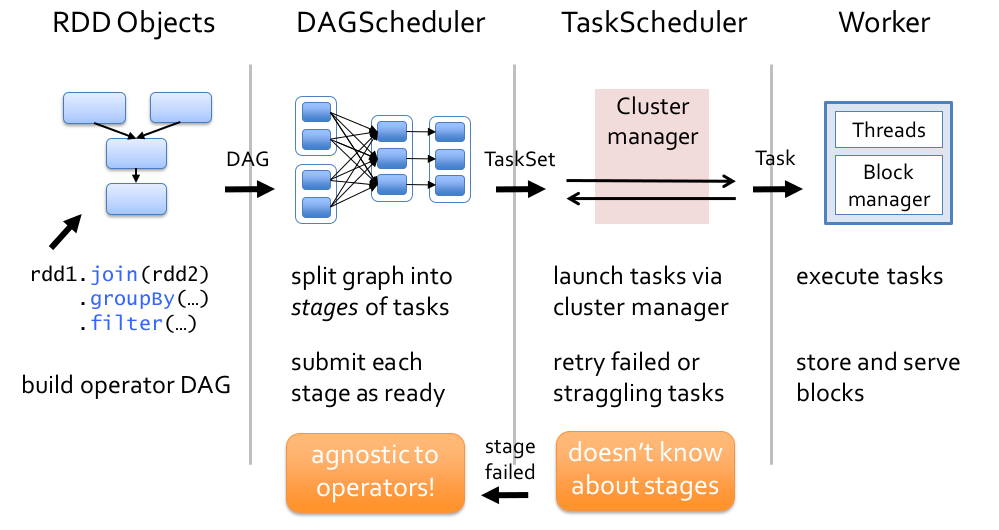
\includegraphics[width=\textwidth]{Figures/spark-job-lifetime.jpeg}
\caption{The lifetime of a Spark job}
\label{fig:lifetime}
\end{figure}

Figure \ref{fig:lifetime} illustrates those four steps clearly.

While the first three steps happen at the driver, the representation of the connection to the Spark cluster, the last step happens at the Executors. We go deeper into each step to understand a Spark Job Lifetime.\\

\textbf{RDD objects creation} Users create RDDs through a set of transformations, at the moment, the RDD is created at the driver.\\
\textbf{DAG Scheduling} When an action is called on an RDD, the RDD is transfered to the next step: DAG Scheduling. It is the process of splitting the DAG into stages, then submitting each stage as ready.
A module called DAGScheduler is in charge of DAG Scheduling. A stage is a set of independent tasks all computing the same function that need to run as part of a Spark job, where all the tasks have the same shuffle dependencies. Each DAG of tasks runs by the scheduler is splitted up into stages at the boundaries where shuffle occurs, and then the DAGScheduler runs these stages in topological order.\\
\textbf{Task Scheduling} TaskScheduler is the component which receives the stages from DAGScheduler and submits them to the cluster.\\
\textbf{Task Execution} Spark calls worker as Executor. The backend will receive the worker list from the Cluster Manager, then it will launchTask at the Executor. A BlockManager at each Executor will help it to deal with shuffle data and cached RDDs. New TaskRunner is created at the Executor and it starts the threadpool to process taskset, each task runs on one thread. After finishing the tasks, results are sent back to the driver or saved to disks.\\

Some information we need to notice are:
\begin{itemize}
\item Thanks to the DAGSchedulerEventProcessLoop, DAGScheduler can keep track of stages’ statuses and resubmit failed stages.
\item TaskScheduler only deals with taskSet after being formed from Stages at DAGScheduler,  that’s why it doesn’t know any thing about stages.
\item A Spark program can contain multiple DAGs, each DAG will have one action. So, inside a driver, they are submitted as jobs one by one in order.
\item Spark has a nice feature appears from version 1.2: dynamic resource allocation. Spark will base on the workload to request for extra resources when it needs or give the resources back to the cluster if they are no longer used.
\end{itemize}

\subsection{The Log Mining Example}

Below is an example about log mining. The idea of the example is loading the log, then we keep the error messages in memory and analyze it many times. By using caching, we can reduce the analyzed times. This is just a basic example to demonstrate how to write a Spark program, and the caching feature in action.

\begin{lstlisting}
//base RDD
val lines = spark.textFile("hdfs://...")

//transform to get error RDD, then cache it.
val errors = lines.filter(_.startsWith("ERROR"))
val messages = errors.map(_.split('\t')(2))
val cachedMsgs = messages.cache()

//action 1
cachedMsgs.filter(_.contains("foo")).count
//action 2
cachedMsgs.filter(_.contains("bar")).count
\end{lstlisting}

Table \ref{trans-act} gives us some basic transformations and actions inside Spark.\\

Firstly, create an RDD by reading an input file. Then we apply a set of transformations: filter and map to get the error logs and preprocessing them by splitting them by tabluture character. Then, we cache it. At the moment the "cache" command is called, nothing happens. When action 1 is happend, Spark keeps the cachedMsgs in memory, then filters the error logs which contains "foo". When action 2 is called, the cachedMsgs was kept in memory so Spark does not need to process everything from the beginning as the action 1 was called. If there are many actions after action 2 and they also process on cachedMsgs, they also do not need to process the previous part from scratch. This reduces the cost of I/O and computation many times.

%----------------------------------------------------------------------------------------
%	SECTION 2
%----------------------------------------------------------------------------------------

\section{Apache SparkSQL}
SparkSQL is a new module of Apache Spark, which provides the flexibilities for users to combine relational programming and functional programming through DataFrame API. It also provides an extensible optimizer called Catalyst, which utilizes the features of Scala language to make it easier to add new rules and to control code generation. The two following subsections brieftly describe these two contributions.\\


\subsection{DataFrame API}
DataFrames are distributed collection of column-structured records which can be manipulated by both new functional API and produceral API of Spark. DataFrames can be created from various data sources or even existing RDDs. 

DataFrame also provides user-defined function, which is very important for database systems. The inline-definition of UDFs also makes it easier for user to write their functions.\\
Each DataFrame object has a 'lazy' logical plan which means no execution occurs until an action is called, this let the logical plan itself have better chance of optimizations.\\ 

Spark SQL supports two different methods for converting existing RDDs into DataFrames:
\begin{itemize}
\item Using reflection to infer the schema of an RDD that contains specific types of objects. This method provides more concise codes and it works well when we already know about the schema of the object.
\item Using a programmatic interface, we can construct a schema and then apply it to an existing RDD. This method is more verbose, it allows us to construct DataFrames when the columns and their types are not known until runtime.
\end{itemize}

\subsection{Catalyst Optimizer}
Catalyst Optimizer is an extensible optimization engine. It contains a general library for representing trees and applying rules to manipulate them.\\
\textbf{Trees} Tree is the main data structure in Catalyst, which is formed by many nodes. A node has a type and its childs, which can be none or more than zero nodes. Node objects are read-only and can be manipulated using functional transformations.\\
\textbf{Rules} Trees can be transformed to another trees by using rules. By utilizing pattern matching, a Scala feature, a part of a tree can be found and replaced by another one.\\

\begin{figure}
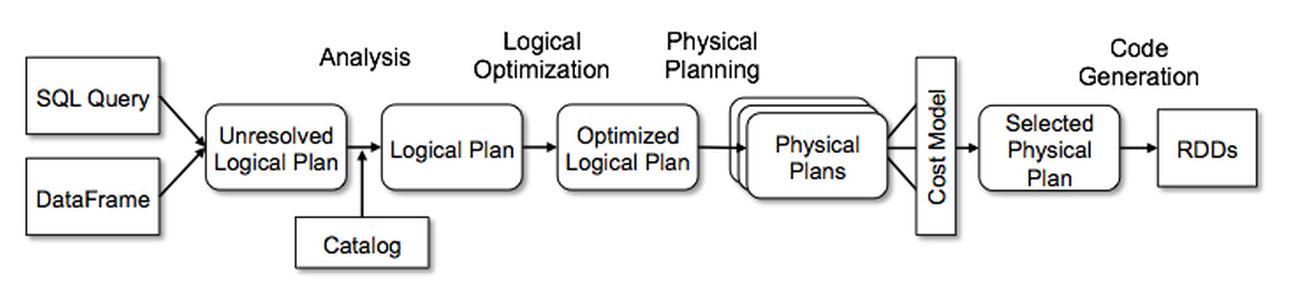
\includegraphics[width=\textwidth]{Figures/catalyst-flow.png}
\label{fig:catalyst}
\caption{Catalyst Dataflow}
\end{figure}

A Catalyst tree transformation process is composed by four phases. Figure \ref{fig:catalyst} illustrates this process. We explain each process below:
\begin{itemize}
\item \textbf{Analysis} Its input is a relation to be computed, which is created from SparkSQL Parser to form an Abstract Syntax Tree (AST) or from using DataFrame API. The relation can contain unresolved attribute references or relations, which means we do not know its type or have not matched it to an input table (or an alias). With Catalyst Rules and a Catalog, an object which is used to keep track of created tables, SparkSQL resolves those attributes.
\item \textbf{Logical Optimizations} This phase applies rule-based optimizations to the logical plan which is outputed from Analysis phase. By utilizing the nature of Scala language,users can simply add rules to fulfill their needs.
\item \textbf{Physical Planning} In this phase, Spark SQL tries to generate as much physical plans as possible from one optimized logical plan, by using physical operators that match the Spark execution engine. By associating to a cost model, it can select the best plan.
\item \textbf{Code Generation} This final phase of query optimization involves generating Java bytecode to run on each machine. By utilizing a special feature of Scala, which is quasiquotes, Catalyst can make code generation simpler. Quasiquotes allow the programmatic construction of abstract syntax trees (ASTs) in the Scala language, which can then be fed to the Scala compiler at runtime to generate bytecode. Again, due to the simplicity of quasiquotes, users can add their own rules for new types of expressions.
\end{itemize}
\subsection{An application written using SparkSQL}
Below is a simple example of SparkSQL to demonstrate the combination of relational programming and functional programming of SparkSQL.\\

\begin{lstlisting}
case class Person(name: String, age: Integer)
val input = sc.textFile("examples/src/main/resources/people.txt")
val people = input.map(_.split(",")).map(p => Person(p(0), p(1).trim.toInt))
val peopleDF = people.toDF()
peopleDF.registerTempTable("people")
val teenagers = sqlContext.sql("SELECT name FROM people WHERE age >= 13 AND age <= 19")
val result = teenagers.map(t => "Name: " + t(0)).collect.foreach(println)
\end{lstlisting}

We can declare our data structure, then read the input file with that format and store into an RDD. We create a DataFrame from that RDD and create a table from it. We are using the method of reflection to interoperate between DataFrame and RDD. An SQL query is passed to SparkSQL. After the optimization and translation happened, a normal Spark Job is created with a Directed-Acyclic Graph inside. An action would trigger all these things.

\begin{table}[]
\centering
\caption{Some transformatios and actions in Spark}
\label{trans-act}
\begin{tabular}{|l|l|}
\hline
\multicolumn{2}{|l|}{Transformation}           \\ \hline
\multicolumn{2}{|l|}{map(f : $T \Rightarrow $U) : $RDD[T] \Rightarrow $RDD[U]} \\ \hline
\multicolumn{2}{|l|}{filter(f : $T \Rightarrow $Bool) : $RDD[T] \Rightarrow $RDD[T]} \\ \hline
\multicolumn{2}{|l|}{flatMap(f : $T \Rightarrow $Seq[U]) : $RDD[T] \Rightarrow $RDD[U]} \\ \hline
\multicolumn{2}{|l|}{sample(fraction : Float) : $RDD[T] \Rightarrow $RDD[T]} \\ \hline
\multicolumn{2}{|l|}{groupByKey() : $RDD[(K, V)] \Rightarrow $RDD[(K, Seq[V])]} \\ \hline
\multicolumn{2}{|l|}{reduceByKey(f : $(V, V) \Rightarrow $V) : $RDD[(K, V)] \Rightarrow $RDD[(K, V)]} \\ \hline
\multicolumn{2}{|l|}{union() : $(RDD[T], RDD[T]) \Rightarrow $RDD[T]} \\ \hline
\multicolumn{2}{|l|}{join() : $(RDD[(K, V)], RDD[(K, W)]) \Rightarrow $RDD[(K, (V, W))]} \\ \hline
\multicolumn{2}{|l|}{cogroup() : $(RDD[(K, V)], RDD[(K, W)]) \Rightarrow $RDD[(K, (Seq[V], Seq[W]))]} \\ \hline
\multicolumn{2}{|l|}{crossProduct() : $(RDD[T], RDD[U]) \Rightarrow $RDD[(T, U)]} \\ \hline
\multicolumn{2}{|l|}{mapValues(f : $V \Rightarrow $W) : $RDD[(K, V)] \Rightarrow $RDD[(K, W)]} \\ \hline
\multicolumn{2}{|l|}{sort(c : Comparator[K]) : $RDD[(K, V)] \Rightarrow $RDD[(K, V)]} \\ \hline
\multicolumn{2}{|l|}{partitionBy(p : Partitioner[K]) : $RDD[(K, V)] \Rightarrow $RDD[(K, V)]} \\ \hline
\multicolumn{2}{|l|}{Actions} \\ \hline
\multicolumn{2}{|l|}{count() : $RDD[T] \Rightarrow $Long} \\ \hline
\multicolumn{2}{|l|}{collect() : $RDD[T] \Rightarrow $Seq[T]} \\ \hline
\multicolumn{2}{|l|}{reduce(f : $(T, T) \Rightarrow $T) : $RDD[T] \Rightarrow $T} \\ \hline
\multicolumn{2}{|l|}{lookup(k : K) : $RDD[(K, V)] \Rightarrow $Seq[V]} \\ \hline
\multicolumn{2}{|l|}{save(path : String) : Outputs RDD to a storage system, e.g., HDFS} \\ \hline

\end{tabular}
\end{table} 
% Chapter Template

\chapter{A Work Sharing Framework} % Main chapter title

\label{Chapter3} % Change X to a consecutive number; for referencing this chapter elsewhere, use \ref{ChapterX}

\lhead{Chapter 3. \emph{Apache SparkSQL}} % Change X to a consecutive number; this is for the header on each page - perhaps a shortened title

%----------------------------------------------------------------------------------------
%	SECTION 1
%----------------------------------------------------------------------------------------

\section{Work Sharing}

In large data ware houses, many queries are usually submitted at the same time by multiple users. In the context of big data, a query would take long time to run. There are some data that would be used more frequently than the others, so we can avoid the redundant computations by sharing works among those queries and reduce the total amount of execution time. \\
The idea of work sharing originally comes from Multiple Query Optimization (MQO) \cite{sellis1988}. There are many works on traditional database systems \cite{cosar1993} \cite{bayir2007} \cite{georgios2012} \cite{stavros2005} and also on Hadoop MapReduce have been published. Olston et al. worked on a system called CoScan \cite{olston2011}, a system for sharing data and processing costs among multi-step MapReduce workflows which are executed in Hadoop. In Apache Pig, a number of work sharing optimizations \cite{pigmqo} have been used with the idea of MQO. The current state-of-the-art work in this field is MRShare\cite{nikiel2010} on Apache Hadoop. With the grouping technique, it provides the map input sharing to share scan of input files and map output sharing for saving cost of communication.\\
%----------------------------------------------------------------------------------------
%	SECTION 2
%----------------------------------------------------------------------------------------

\section{SparkSQL Server}
All the works above are only supported for Hadoop MapReduce and they are focused only on a part of work sharing, then they are hard to extend when users want to have new sharing techniques. To the best of our knowledges, there is no published work about Multi Query Optimization on Apache Spark. In our work, we present a new framework called SparkSQL Server, which is focused on work sharing among multiple queries.\\

SparkSQL Server supports queries written in SQL by using DataFrame API of SparkSQL or in produceral languague supported by SparkCore itself.\\

The framework does not only care about work sharing among multiple queries but also the scheduling mechanisms to associate with the sharing techniques or to fullfil the users' requirements.\\

The framework is generalized so it can support many types work sharing. All the modules of SparkSQL Server are easy to extend, this lets users and developers easily plug their own implementations into the framework.\\

\subsection{System Design}
The design of our framework aims at the generalization and extensibility so users and developers can easily plug their own implementations. Figure \ref{fig:sparksql-design} expresses the design of our system.\\
\begin{figure}
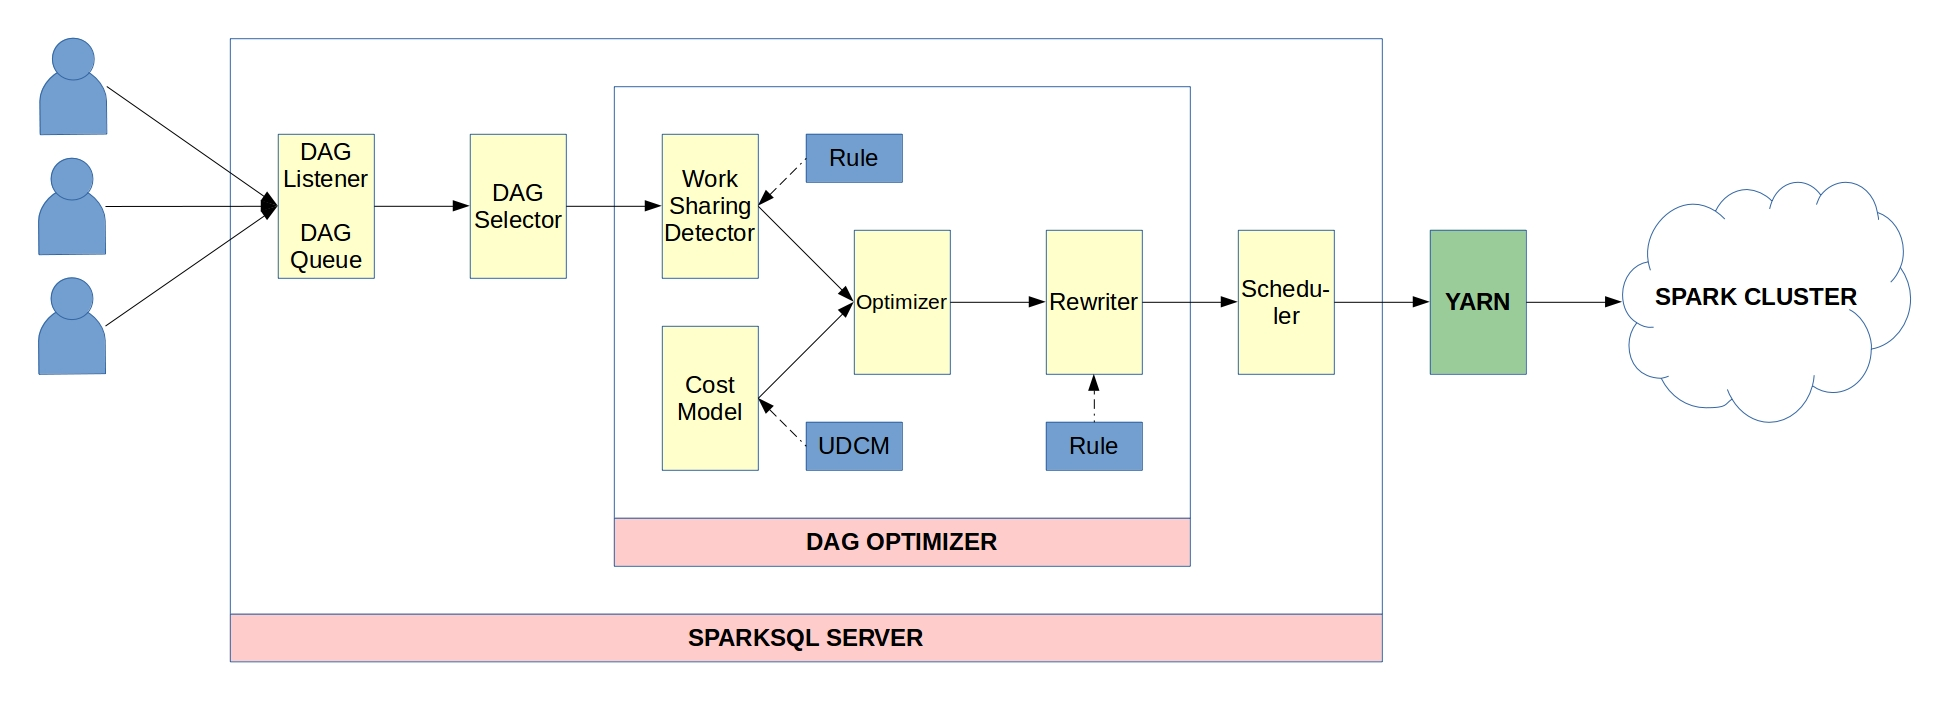
\includegraphics[width=\textwidth]{Figures/sparksql-server-design.jpg}
\label{fig:sparksql-design}
\caption{The design of SparkSQL Server}
\end{figure}

In overall, our framework has two sides: client side and server side.\\
\textbf{Client side} The client submits the query and needed information to SparkSQL Server so SparkSQL Server can reconstruct exactly the query happened at client side. The query can be written by using produceral operations in Spark or relational operations in SparkSQL or the combination of both types of operations.\\
\textbf{Server side}  The SparkSQL Server contains three main components:\\
\begin{itemize}
\item The Listeners, which are listened to client connections and communicate with them.
\item The DAG Optimizer are the hearts of our framework. All the detections, optimizations, and transformations happen here. The DAG Optimizer is composed of:
\begin{itemize}
\item WorkSharing Detector: this module detects the sharing opportunities among a batch of jobs which has just received from clients. The detector uses the rule-based mechanism to detect the sharable jobs. Users can easily write their own rules to detect sharable jobs with many types of sharing.
\item CostModel: it calculates the cost of each execution plan. Users provide their own cost model by the User-defined Cost Model.
\item Optimizer: it receives the input from the output of WorkSharing Detector and uses the CostModel to pick the best plan to execute.
\item Rewriter: the Rewriter transforms the original execution plans into the optimized execution plans and then submits them to the Schedulers. The transformation is also based on the rule-based mechanism. It is very easy to define a new rule to support another type of sharing.
\end{itemize} 
Again, all of these four modules are extendable so users can plug their owns into these modules.
\item The Schedulers, which are used to fulfill users' requirements and to associate with the sharing techniques. These Schedulers are aslo extendable so users can plug their own shechuling strategies.
\end{itemize}

\subsection{Implementations}
Similar to the above subsection, we present the implementations of our framework on both client side and server side. The order of the explaination is the same as the flow in figure \ref{fig:sparksql-design}.\\
\textbf{Client side} We will modify the spark-submit command so that it will not send the application to the cluster manager but to the SparkSQL Server, using this option:  --sparksql-server\\
Each client starts it own driver with its own SparkContext. Then, the client can generate its DAG, the DataFrame creation and send those information: DAG, DataFrame generation, SQL Query to the SparkSQL Server.\\
The client needs to send the jar file, because it contains all user defined functions, classes which are very important to reassemble the DAG at server side. It also needs to sends needed information so the SparkSQL Server can reconstruct the DAG and the query. Don’t forget that the query has already been optimized by Catalyst at the client side.\\
\textbf{Server side}
\begin{itemize}
\item \textbf{DAG Listener and DAG Queue} DAG Listener will accept the clients’ connections and receive DAGs, queries and other information they send. Then, it passes to the DAG Queue, the DAG Queue accepts the information the clients send at the FIFO order. In this component, the full DAG of each user will be built based on the initial DAG, the DataFrame creation information and the query. The DAG Queue has a window with fixed size, after reaching the size of the windows, DAG Queue will send a batch of DAGs (and queries also) into the next components. The window size right now is fixed as a constant, it will be changed when we take care of scheduling.
\item \textbf{DAG Selector} This component is something called a pre-scheduler, which will based on the constraint attached with each query to fulfill user’s requirements. For example: job submitted with a deadline. Right now, it just uses the simple FIFO strategy.
\item \textbf{Worksharing Detector} This component will detect which DAGs have the opportunity for worksharing, which DAGs haven’t. Remember that worksharing here is not only sharing scan, it can also have other variants such as sharing group-by or join. It works as rule-based mechanism to detect the worksharing opportunity. 
\item \textbf{Cost Model} It provides an interface so that users can plug their own cost model, which is called User defined cost model, into the system.
\item \textbf{Optimizer} With a bag from the output of the previous and a cost model associated with its sharing type, the Optimizer component will do the job: pick the plan with the lowest cost.
\item \textbf{Rewriter} This component has many families of rewrite. Each family will have many rewrite rules. It will generate a rewritten DAG which can be optimized, and use the rule that Optimizer picked to transform the original DAGs into the new ones..
\end{itemize}

\subsection{An Example on SparkSQL Server}

This section gives us an example of SparkSQL Server in action so we can understand how SparkSQL Server works clearly.
Three examples below are similar to the example in section 2.2.3 and we focus only on scan sharing in this example. The explaination has three parts for each components: Input, Output, and we relate them to the example.\\
\textbf{User1}

\begin{lstlisting}
case class Teacher(name: String, age: Integer)
val input = sc.textFile("hdfs://A.txt")
val people = input.map(_.split(",")).map(p => Teacher(p(0), p(1).trim.toInt))
val peopleDF = people.toDF()
peopleDF.registerTempTable("people")
val teacher = sqlContext.sql("SELECT name FROM people WHERE age <= 50")
val result = teacher.map(t => "Name: " + t(0)).collect.foreach(println)
\end{lstlisting}

\textbf{User2}

\begin{lstlisting}
case class Student(fullname: String, age: Integer)
val input = sc.textFile("hdfs://A.txt")
val people = input.map(_.split(",")).map(p => Student(p(0), p(1).trim.toInt))
val peopleDF = people.toDF()
peopleDF.registerTempTable("people")
val student = sqlContext.sql("SELECT name FROM people WHERE age >= 19")
val result = student.map(t => "Name: " + t(0)).collect.foreach(println)
\end{lstlisting}

\textbf{User3}

\begin{lstlisting}
case class Person(name: String, age: Integer)
val input = sc.textFile("hdfs://B.txt")
val people = input.map(_.split(",")).map(p => Persion(p(0), p(1).trim.toInt))
val peopleDF = people.toDF()
peopleDF.registerTempTable("people")
val adults = sqlContext.sql("SELECT name FROM people WHERE age >= 25")
val result = adults.map(t => "Name: " + t(0)).collect.foreach(println)
\end{lstlisting}

\textbf{Client Side}
\begin{itemize}
\item Input: Users’ applications (jar files)
\item Output: Jarfile, DAGs, DataFrame creation information, SQL queries are sent to SparkSQL Server. In those example, we have DAG1, DAG2, DAG3.
\end{itemize}

\textbf{Server Side}\\
\textbf{DAG Listener and DAG Queue}
\begin{itemize}
\item Input: DAGs and queries from clients
\item Output: Batch of DAGs, queries, DataFrame creation information after reaching the window size of DAG Queue
\item In the example, let assume the window size of DAG Queue is 3, so the output will be DAG1, DAG2, DAG3. If there is user4 submits the job, it will be packed with another two jobs.
\end{itemize}

\textbf{DAG Selector}
\begin{itemize}
\item Input: Batch of DAGs
\item Output: Batch of DAGs based on scheduling strategies (FIFO at the moment).
\item In the example, the input and the output is the same as we use FIFO strategy.
\end{itemize}

\textbf{Worksharing Detector}
\begin{itemize}
\item Input: Batch of DAGs
\item Output: Bags of DAGs which are labeled each type of sharing (sharing scan, sharing groupby…) or "no sharing".
\item In the example, we got two Bags: DAGBag1: {DAG1, DAG2} with the label: “scan sharing”; DAGBag2: {DAG3} with the label: "no sharing".
\end{itemize}

\textbf{Cost Model}
\begin{itemize}
\item Input: a DAG and its metadata to compute the cost
\item Output: costs belong to DAGs
\item In the example, we use the MRShare Cost Model so it returns a bag of DAG which can be merged together which is DAGBag1: {DAG1, DAG2}.
\end{itemize}

\textbf{Optimizer}
\begin{itemize}
\item Input: Bags of sharable DAGs, a Cost Model associated to the sharing type of each bag.
\item Output: Bags of optimized DAGs.
\item In the example, we got DAGBag1: {DAG1, DAG2}, DAGBag2: {DAG3}
\end{itemize}

\textbf{Rewriter}
\begin{itemize}
\item Input: Optimized Bags of DAGs
\item Output: Rewritten Bags of DAGs
\item In the example, since MRShare uses the simultaneous pipeline technique to merge jobs, we got DAGBag1: {DAG12}, DAGBag2: {DAG3}
\end{itemize}

\textbf{PostScheduler}
\begin{itemize}
\item Input: Rewritten Bags of DAGs
\item In the example, we got 2 Bags of DAGs. Since the execution order does not affect these jobs or in other way, they are independent on each other, so we just use FIFO strategy to submit to the cluster.
\end{itemize}

The example is only for scan sharing and just to show the dataflow of SparkSQL Server but the system is generalized and extensible so other sharing techniques can be embedded into the system.
% Chapter Template

\chapter{SparkSQL Server in Practice: Scan Sharing} % Main chapter title

\label{Chapter4} % Change X to a consecutive number; for referencing this chapter elsewhere, use \ref{ChapterX}

\lhead{Chapter 4. \emph{SparkSQL Server in Practice: Scan Sharing}} % Change X to a consecutive number; this is for the header on each page - perhaps a shortened title

%----------------------------------------------------------------------------------------
%	SECTION 1
%----------------------------------------------------------------------------------------

\section{Scan Sharing}

In large data warehouses, companies, users submit their queries at the same period of time. There are some files which are "hotter" since they are used more frequently than the others, then reading those files multiple times from disk can be redundant by reading each file only one time and many others users can use them. Sharing scan does not only help to reduce the reading cost but also the communication cost, then the total execution time of the queries is reduced.\\

We embed the sharing scan technique into our framework by using two techniques, one from MRShare works and the other is a feature of Spark itself. Both techniques are easily to embed into our system, this proves the generalization and extensibility of our framework.

%-----------------------------------
%	SUBSECTION 1
%-----------------------------------
\subsection{Current State-of-the-Art}

As described before,  on Apache Spark, there is no published work on Work Sharing. The current State-of-the-art of Scan Sharing on Apache Hadoop MapReduce is MRShare.\\
MRShare is a sharing framework, which provides two techniques of sharing: map input sharing and map output sharing. The idea of MRShare is group the jobs which can share map input or map output into groups, with the constrains of maximizing the total saving.\\

Grouping jobs into one is not always beneficial since the reading cost is decreased but the amount of data shuffled over networks is increased. Using dynamic programming and a cost model, MRShare evalutates possible groups and decides which groups give it the maximum saving.\\
The technique that MRShare uses to merge multiple jobs into one called simultaneous pipeline. It attaches a tagging in each tuple to identify which job it belongs to.\\
%-----------------------------------
%	SUBSECTION 2
%-----------------------------------

\subsection{New Approach for Scan Sharing on Apache Spark}

%----------------------------------------------------------------------------------------
%	SECTION 2
%----------------------------------------------------------------------------------------

There is a fancy feature on Apache Spark which is Caching. This feature utilizes the memory storage to keep data in memory and uses it multiple times. When multiple jobs in a Spark Application using the same input file, we can cache the partitions which are hold the input file at the first job. When the second job wants to do some transformations on those partitions, it does not need to recompute from scratch to get them, it just checks if they are in memory or not, if they are in memory, it gets them and applies transformations on them.\\

Caching is a costly operation itself. If the cost of caching is larger than the cost of reading input files multiple times, so caching is not beneficial. In addition, if memory storage of the cluster is not large enough to cache the whole input files, it may write a part of the input files to disk and read them when needed, which also increases the I/O cost.\\

\section{Scan Sharing in SparkSQL Server}
We integrate two techniques of scan sharing: using MRShare and using caching. \\
\textbf{At client side}, since MRShare requires some pre-defined parameters about the jobs, when users submit their Spark applications through the spark-submit command, they need to pass those parameters too.\\

\textbf{At server side}, we only discuss about the components that we need to plug our own implementations for scan sharing:
\begin{itemize}
\item WorkSharing Detector: we need to add our own Rule which is "ScanSharing" to detect which jobs can be shared scan.
\item CostModel: for MRShare, we implement the cost model that was published in the paper. For caching technique, currently, there is no pulished works about cost model relates to caching data in memory so we do not add the cost model for caching.
\item Optimizer: for MRShare, the dynamic programming algorithms are implemented as described in the paper. Since we do not have the cost model for caching technique, currently, we just output the same batch of jobs as the same as the input batch of jobs.
\item Rewriter: We add two Rewrite rules. For MRShare, we add the simultaneous rewrite rule. For caching, we add the caching rewrite rule. The details of the implementations of simultaneous pipeline technique is described in the next section. The rewrite rule for caching is simple since we cache scan RDD of the first job in the batch, then replace the scan RDD of the rest jobs in the batch with the cached scan RDD.
\item PostScheduler: At the moment, we use FIFO strategy for MRShare technique, while in caching technique, it should be noticed that the first job which does the caching of scan RDD needs to be executed first, then we apply FIFO strategy for the rest jobs in the batch.
\end{itemize} 

\section{Implementations}

Caching is a feature of Apache Spark which is widely used. Besides that, the cost model and dynamic programming algorithms are well described in the MRShare paper. In this section, we just discuss about how we implement the simultaneous pipeline technique used in MRShare.

\subsection{Simultaneous Pipeline Technique}

In general, this technique is used when merging multiple jobs read the same input file into one meta job. The technique has been used in Multi Query Optimization of Apache Pig. In MRShare, they proposed this technique on Hadoop MapReduce as an automatic module. On Apache Spark, to the best of our knowledges, all the query optimizations are currently focusing on single query, not multi query. We reintroduce the simultaneous pipeline technique and implement it on Apache Spark.

There are 4 new RDDs that we create to implement the technique.
\begin{itemize}
\item MuxRDD: The MuxRDD is used to buffer the input record and multiplex it into multiple pipelines, which represent multiple jobs.
\item LabellingRDD: The LabellingRDD is used to attach the label into each tuple before it is shuffled over the network. The label is an integer which is attached to the key of the tuple. So, the old tuple [Key, Value] becomes [(Label, Key), Value].
\item DispatchRDD: The DispatchRDD is used to route the tuple to the right pipeline by using the label attached inside it.
\item PullRDD: Because Spark is based on Pull Mechanism, which means the child RDD asks its parent RDDs to give it the tuple. In default, the saveAsTextFile action has the puller to trigger the job. To keep Spark at it is, we create our new puller called PullRDD.
\end{itemize}

We also modify some parts of the shuffle component on Apache Spark:
\begin{itemize}
\item ShuffledRDD: the ShuffledRDD contains only one Aggregator, the object holds the aggregate function. In our case, to merge multiple jobs which have different Aggregators, we create a list of Aggregators to hold their Aggregators.
\item ExternalSorter: before writing to files and shuffling them over the network, Spark does a local aggregation (it is a combiner in Hadoop MapReduce), so we also need to apply the correct aggregate function to the tuple by checking the label attached into it.
\item AppendOnlyMap: when the aggregation happens in the other stage after getting the data over the network (in Hadoop MapReduce, it is the Reduce phase), again, we need to apply the correct aggregate function to the list of tuple by checking the label attached into it.
\end{itemize}

We provide two examples to demonstrate how simultaneous pipeline technique works. Two jobs are described at two figures below. For each figure, on the left are two original DAGs and on the right is the meta DAG which is merged from those two DAGs.
\begin{itemize}
\item Two jobs, each job has only one ShuffleRDD
From figure \ref{fig:simplemetajob}, we can see the metajob is a DAG which is mainly composed from the two original DAGs. The MuxRDD is attached right after the scan RDD, it does the multiplexing the input into two pipelines. Before going to the ShuffleRDD, a LabellingRDD is inserted right before the ShuffleRDD to attach the label into each tuple. In this example, we have two jobs, so the label has two values which is 0 and 1. The ShuffledRDD is modified so it contains two aggregate functions. The aggregation before and after shuffling happens on the correct tuple with the correct aggregate function due to the label attached into each tuple. The DispatchRDD is attached after the ShuffledRDD and routes the correct tuple to the associated pipeline by the label attached into each tuple. The PullRDD is inserted at last to do the pull and trigger the whole job, then saves the output to disk storage.
\item Two jobs, one job has two ShuffleRDDs
The part of DAG1 from the beginning up to the second ShuffledRDD and DAG2 are merged as the same way as the case above. The difference is that the PullRDD just saves a part of data comes from the pipeline of DAG2, PullRDD is also followed by the rest part of DAG1 and saves to disk storage when finishes. The process is described in figure \ref{fig:complexmetajob}

\begin{figure}
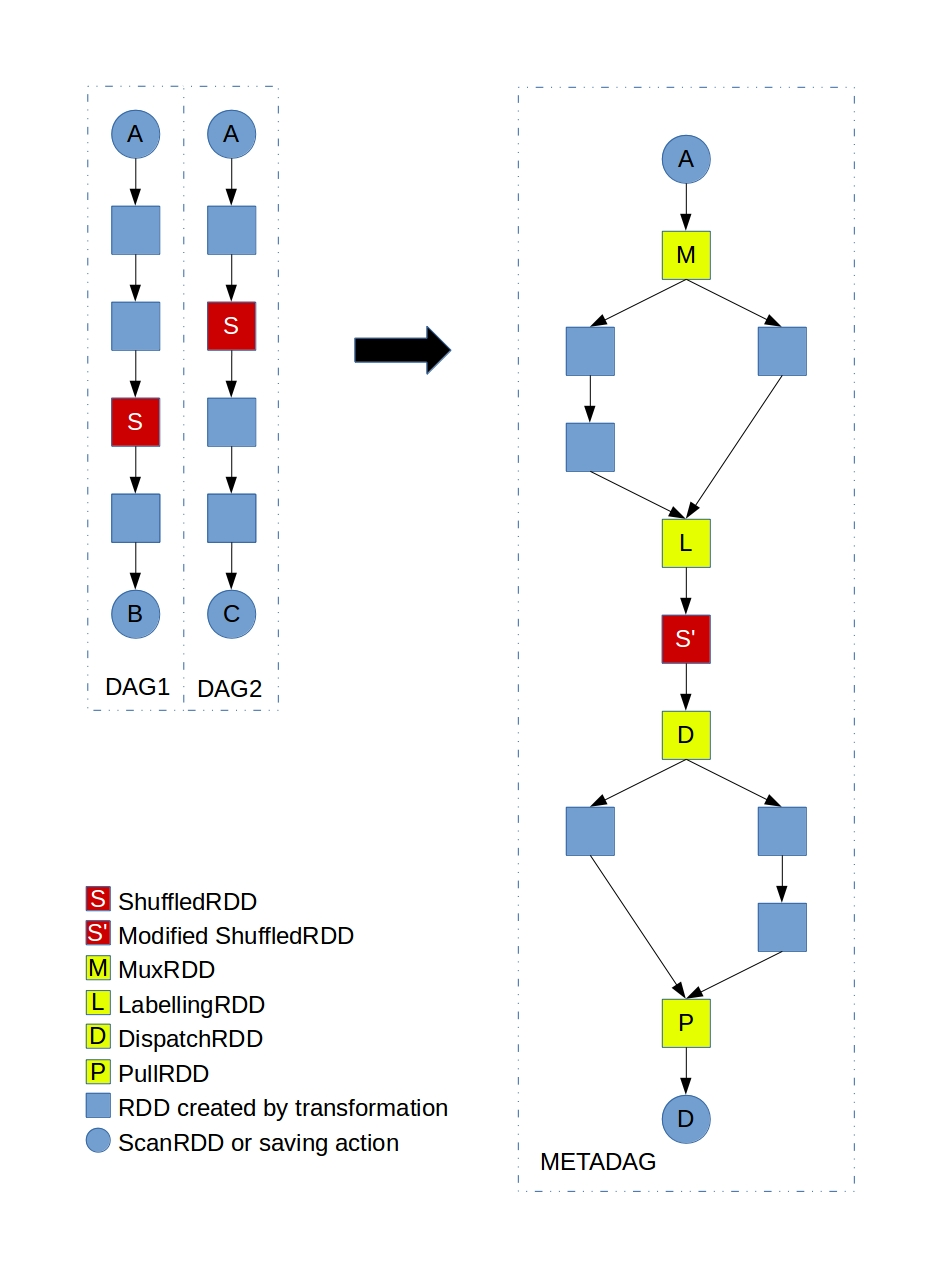
\includegraphics[width=\textwidth]{Figures/singlemetajob.jpg}
\label{fig:simplemetajob}
\caption{Transformation process of a simple case}
\end{figure}

\begin{figure}
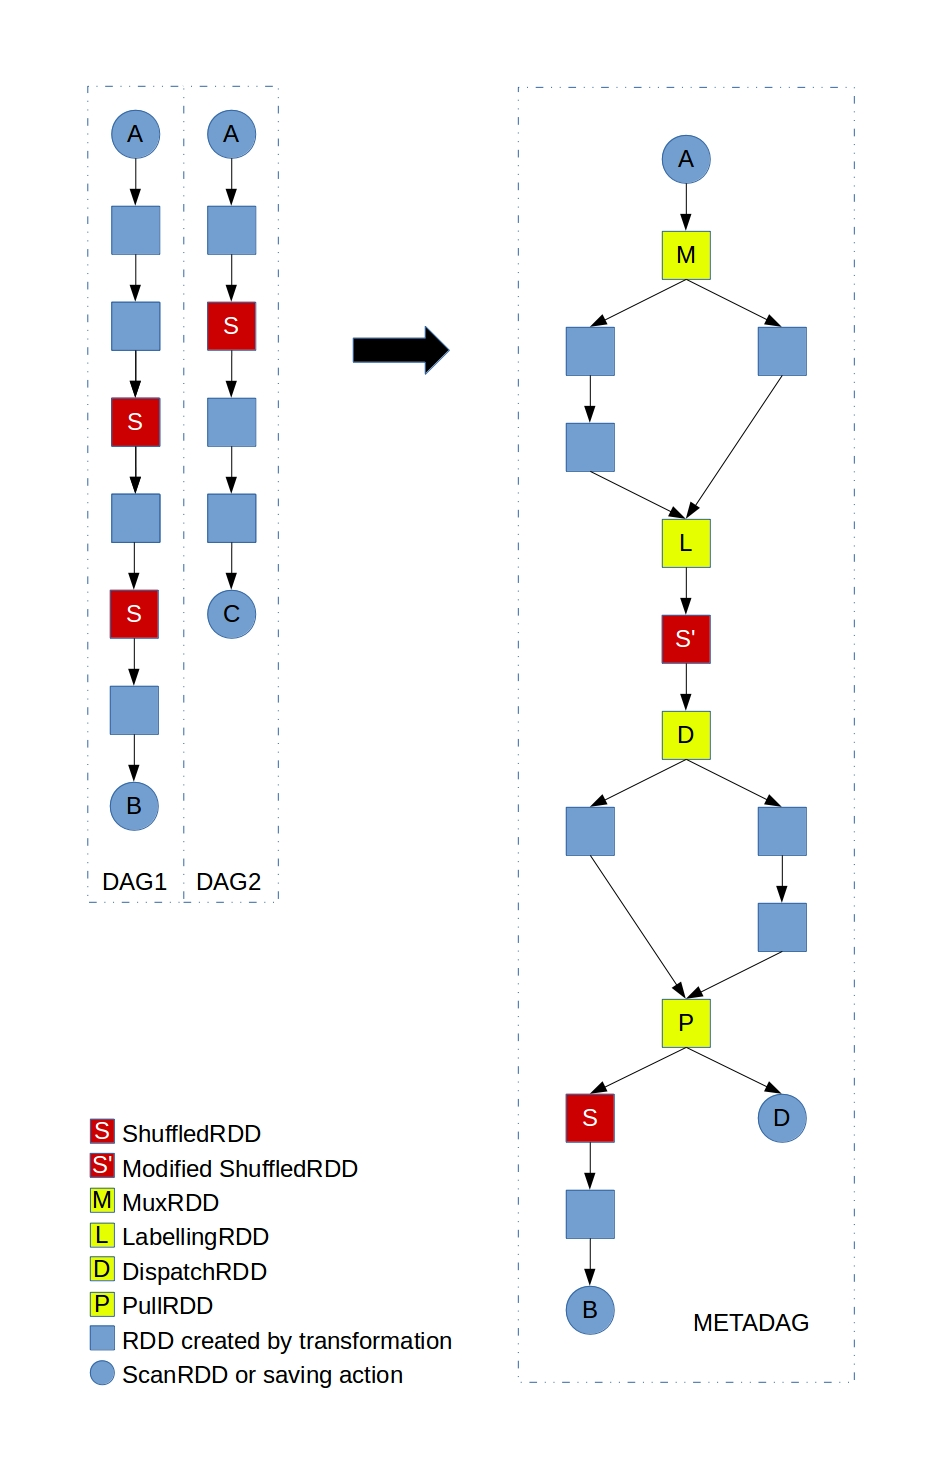
\includegraphics[width=\textwidth]{Figures/complexmetajob.jpg}
\label{fig:complexmetajob}
\caption{Transformation process of a complex case}
\end{figure}
\end{itemize}

This technique is embedded into Spark Source Code and is an automatic feature of SparkSQL Server. In those two examples, we just discuss about two simple cases that can happen when using MRShare and simultaneous pipeline technique, but the more complex DAGs can also be merged into one meta job automatically. 
% Chapter Template

\chapter{Experimental Evaluation} % Main chapter title

\label{Chapter5} % Change X to a consecutive number; for referencing this chapter elsewhere, use \ref{ChapterX}

\lhead{Chapter 5. \emph{Experimental Evaluation}} % Change X to a consecutive number; this is for the header on each page - perhaps a shortened title

This chapter's purpose is to verify the correctness and the efficiency of SparkSQL Server. Due to the limitation of time, in its current state the experiment is designed to be simple. We design the experiments on sharing scan with an input file of 10GB and various Window size of the DAG Queue at SparkSQL Server on two techniques: caching of Spark and sharing map input of MRShare.\\
From these experiments, we evaluate the performance of caching technique and also verify the performance of sharing map input of MRShare, which originally works on Apache Hadoop Mapreduce, on Apache Spark.


%-----------------------------------
%	SUBSECTION 1
%-----------------------------------
\section{Experimental Setup}
Our experimental evaluation is done on a YARN cluster with 17 nodes, each has 4 vcores and 6GB of RAM. Our Apache Spark is modified from version 1.3.1. All results shown in the following are the average of 5 runs: the standard deviation is smaller than 2.5 "\%", hence – for the sake of readability – we omit error bars from our figures.\\
The input files we use are taken from Project Gutenberg, which provides a collection of full texts of public domain books. The size of the input file is 10GB. We take the common used WordCount program for both caching experiment and grep-WordCount for MRShare technique experiment since the paper on MRShare also used grep-WordCount to evaluate their works. We choose the Window Size of the Queue at SparkSQL Server with 2 then 5 and 10.\\
We compare the total runtime of batch of jobs after going through SparkSQL Server and that batch of jobs which is executed one by one without using scan sharing optimization.

%-----------------------------------
%	SUBSECTION 2
%-----------------------------------

\section{Results and Evaluations}
\begin{figure}
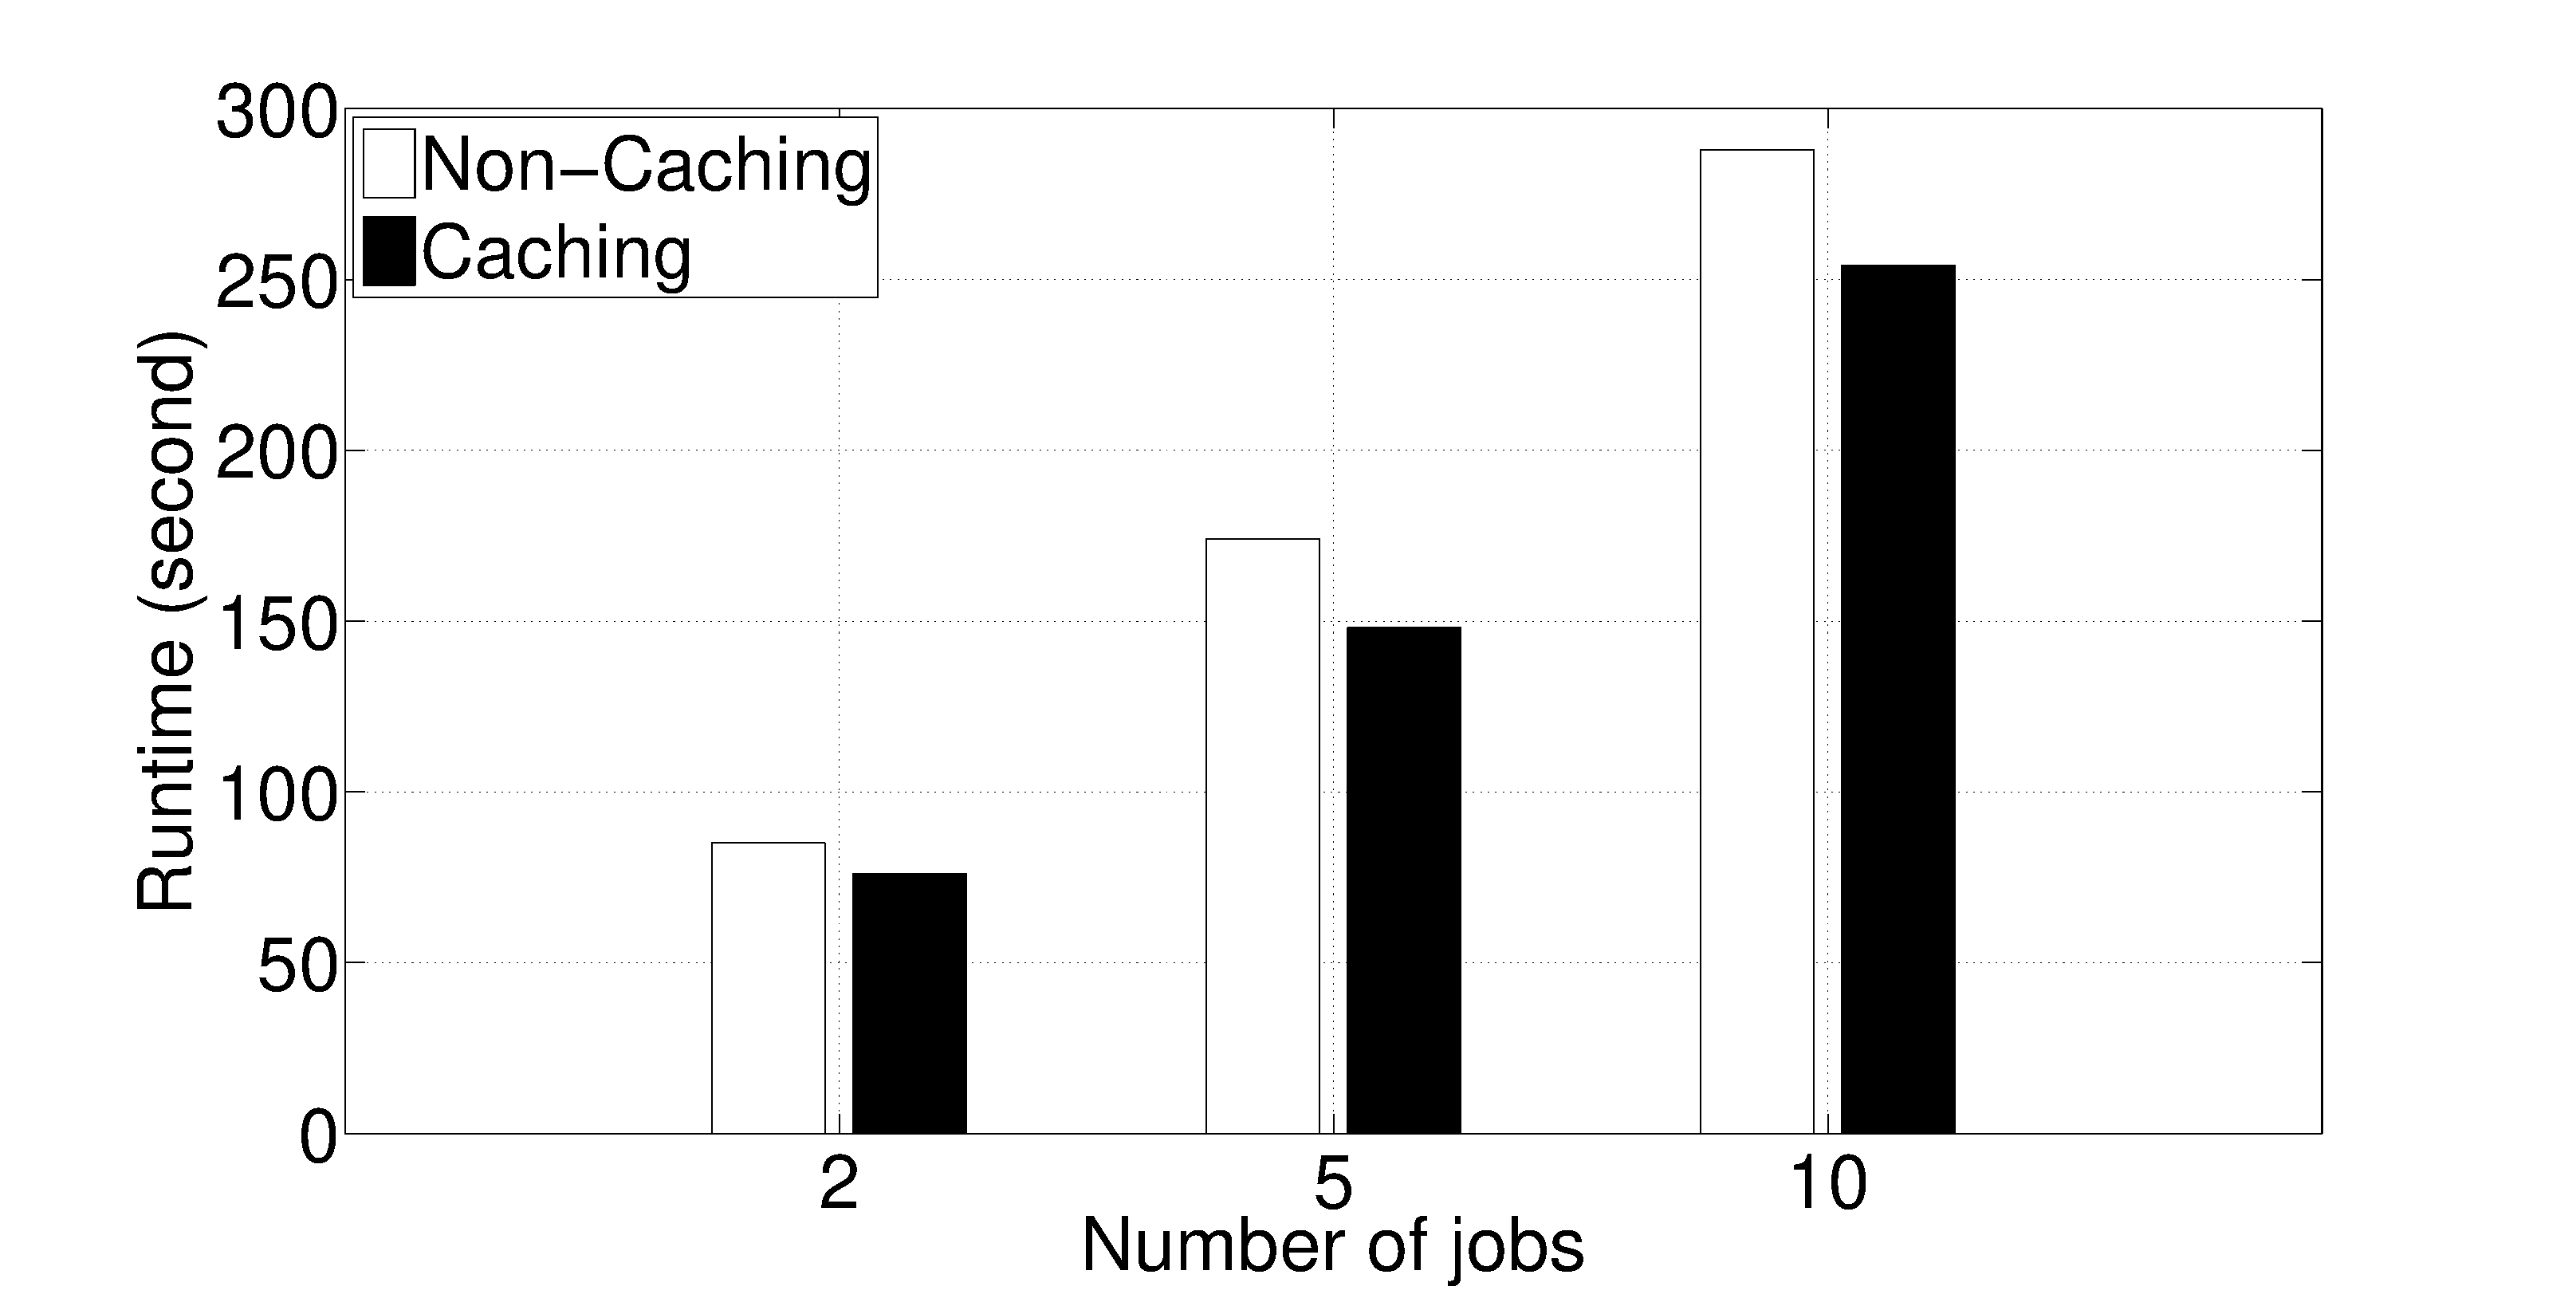
\includegraphics[width=\textwidth]{Figures/caching-vs-non-caching.eps}
\label{fig:caching}
\caption{Performance comparison with jobs submitted by SparkSQL Server and by users, using Caching}
\end{figure}

\begin{figure}
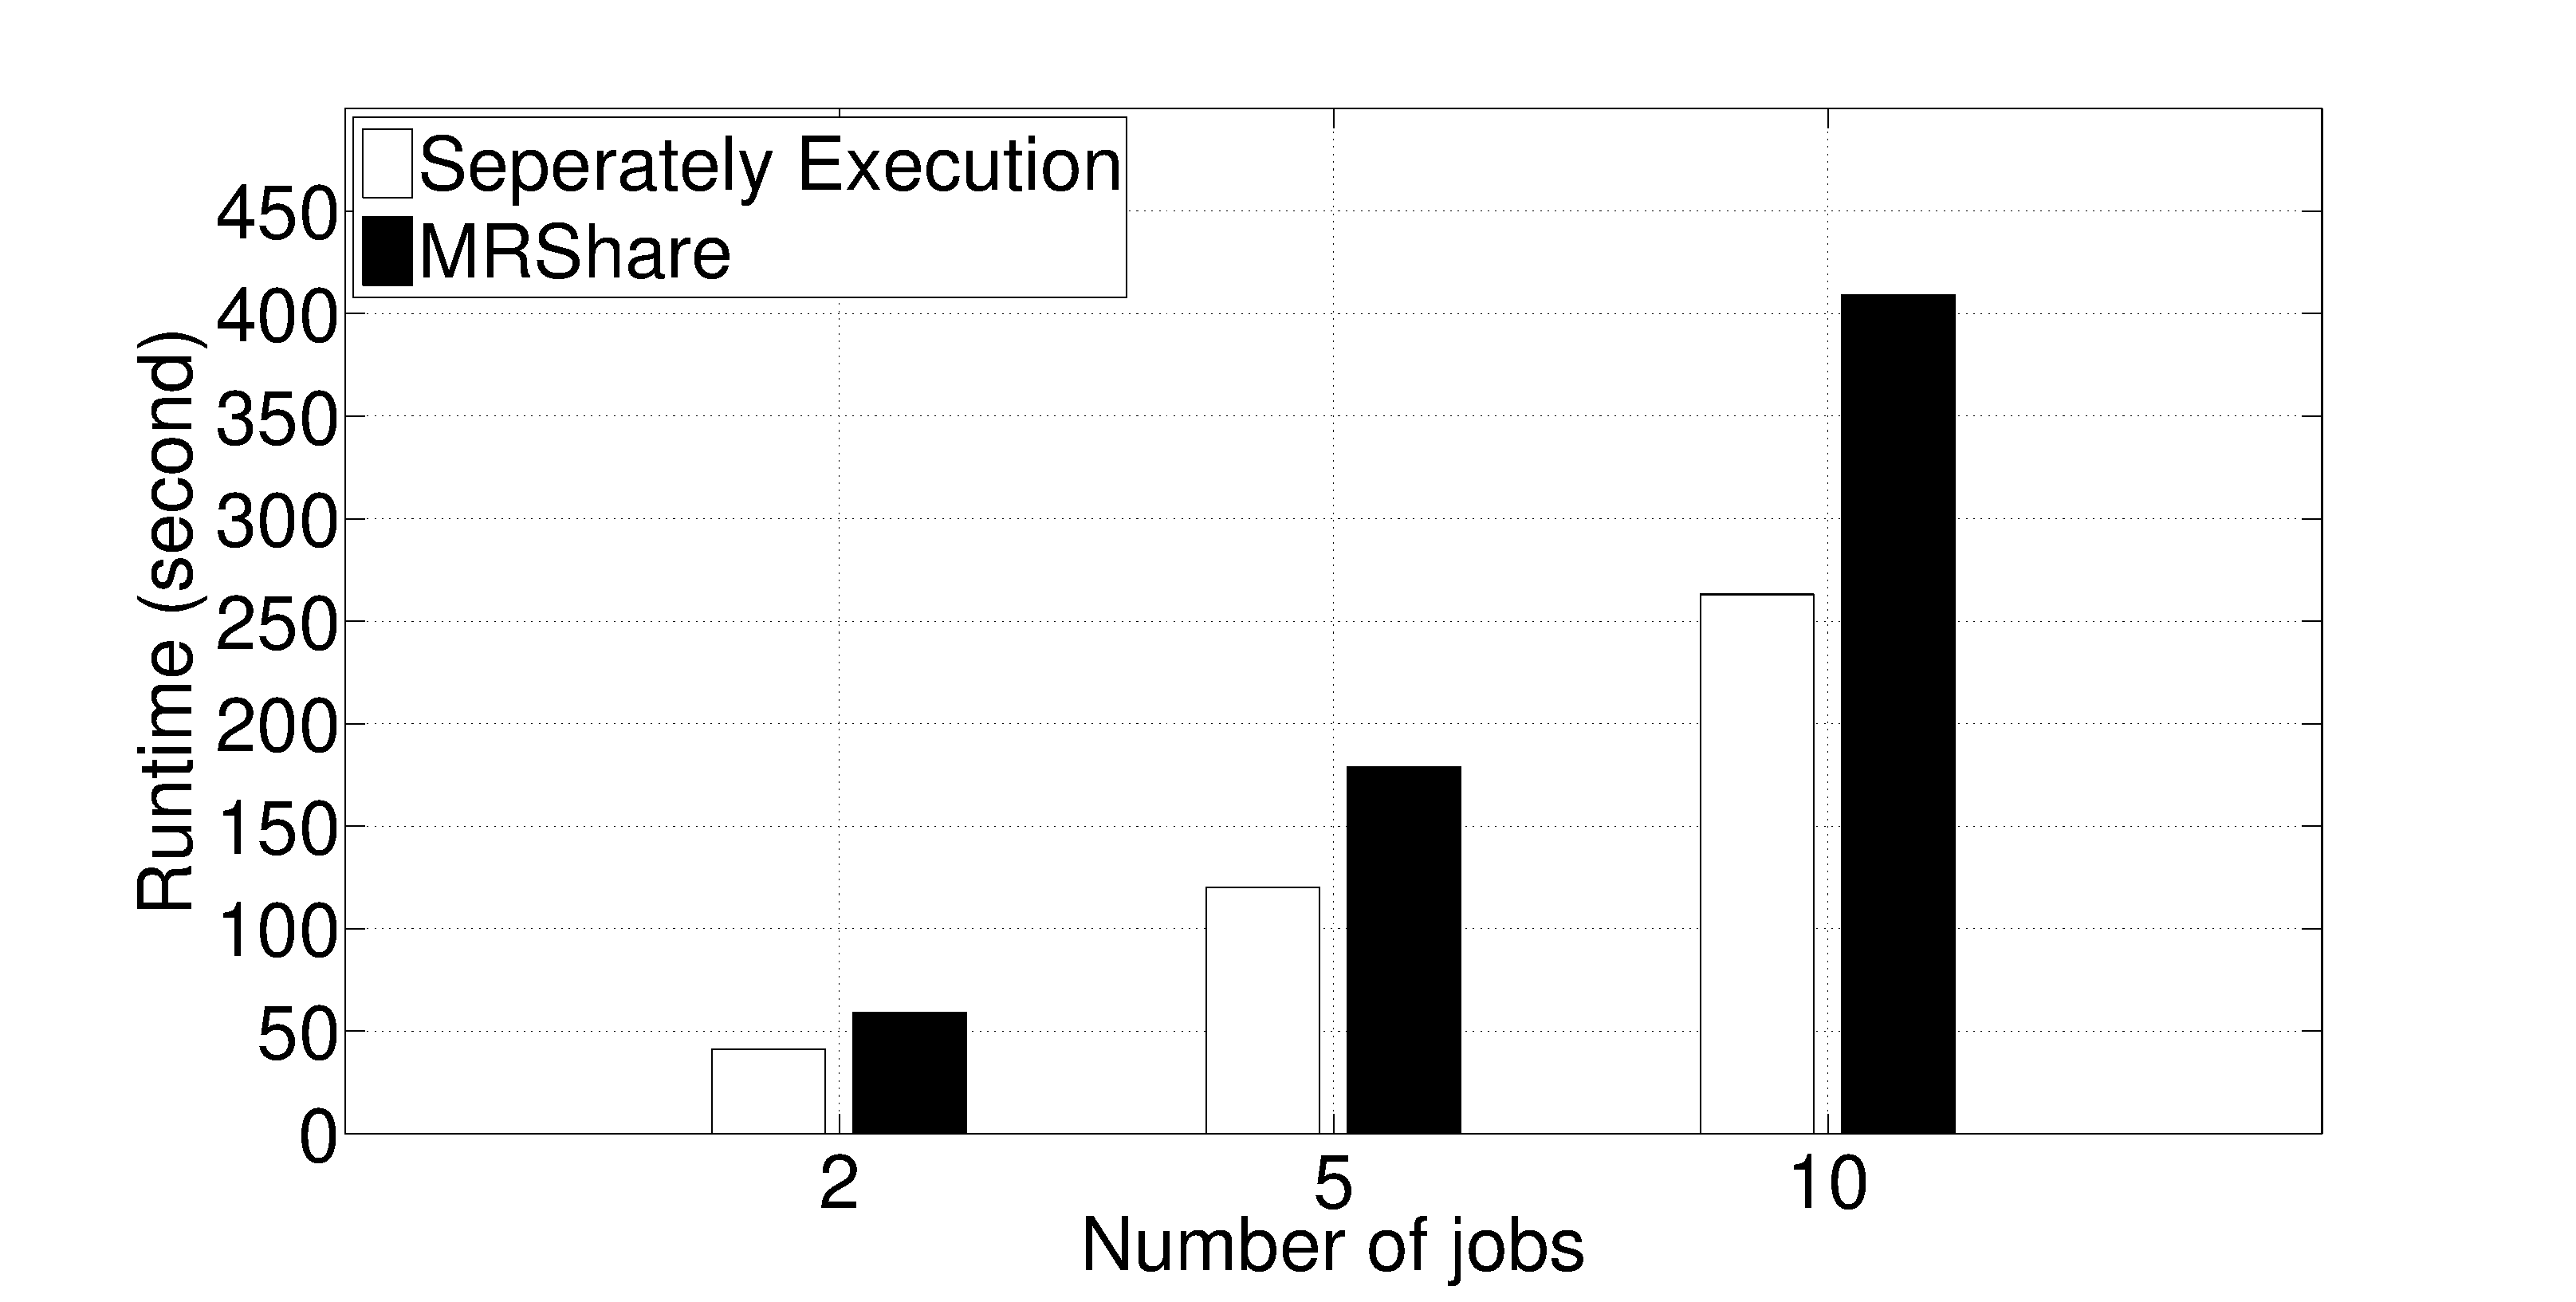
\includegraphics[width=\textwidth]{Figures/multi-mrshare.eps}
\label{fig:mrshare}
\caption{Performance comparison with job submitted by SparkSQL Server and by users, using MRShare}
\end{figure}

With caching technique, as illustrated in figure \ref{fig:caching} for number of jobs varies from 2 to 10, batch of jobs going through SparkSQL Server has total runtime smaller than those jobs which are executed seperately. The saving using caching is not large in comparison to the total amount of time. This means that the sharing scan benefits do not dominant the sharing of computations. The SparkSQL Server functions well and gives the better performance rather than running those jobs submitted by users seperately.\\

Figure \ref{fig:mrshare} describes the performance of jobs submitted by SparkSQL Server and by users, using MRShare sharing technique. With sharing map input technique of MRShare. The total runtime of batch of jobs submitted by SparkSQL Server is larger than the total runtimes of those jobs submitted separately by users. The larger number of jobs are merged into a group, the larger total runtime it is. There are two reasons to explain this result and they are not related to the SparkSQL Server:\\
\begin{itemize}
\item In Apache Spark, a tuple  is immutable. So, when we do the tagging, we can not modify directly on the original tuple but need to generate a new tuple. We create too many objects and the Garbage Collector needs to take more time to do it job. MRShare produces 1 meta jobs for 2 jobs submitted, 2 meta jobs which are created by merging 2 and 3 seperated jobs, and 3 meta jobs which are created by merging 3, 3 and 4 seperated jobs. We sum the average of garbage collector runtime of those meta jobs and also sum the average of garbage collector runtime of seperated jobs. Table \ref{gc-runtime} shows the average of Garbage Collector runtime between MRShare technique and executing jobs separately. The more jobs are merged into a single meta job, the larger the average of garbage collector runtime is. In Apache Hadoop MapRedue, the record is mutable so it can reduce the cost of Garbage Collector.
\item The tagging operation is also a costly operation since larger data is shuffled over the network. We make a simple experiment by creating a Spark application that we manually replicate the input tuple and tag the labeling into it. The number of replications is also varied from 2 then 5 and 10. The total runtime of MRShare technique is equal or smaller than the total runtime of executing jobs seperately, which means that the tagging technique is a costly operation. The original works of MRShare does not include the tagging cost into their cost model although through experiments, we realize that the cost of tagging is not negligible.
\end{itemize}

\begin{table}[]
\centering
\caption{Garbage Collector Average Runtime}
\label{gc-runtime}
\begin{tabular}{|l|l|l|}
\hline
Number of jobs & Seperately executed & MRShare \\ \hline
2              & 23 ms                  & 200 ms    \\ \hline
5              & 63 ms                  & 700 ms    \\ \hline
10             & 131 ms                 & 1800 ms   \\ \hline
\end{tabular}
\end{table}

The result of MRShare technique shows that the MRShare does not work as well as it does on Hadoop MapReduce since it is originally designed for MapReduce. In other words, the simultaneous pipeline technique that MRShare for Hadoop MapReduce uses is not suitable on Apache Spark due to the nature of each framework.\\

From both experiments, the SparkSQL Sever proves its correctness. It also shows the extensibility of the framework since we can easily add new sharing technique into the framework. 
% Chapter Template

\chapter{Contributions and Future Works} % Main chapter title

\label{Chapter6} % Change X to a consecutive number; for referencing this chapter elsewhere, use \ref{ChapterX}

\lhead{Chapter 6. \emph{Contributions and Future Works}} % Change X to a consecutive number; this is for the header on each page - perhaps a shortened title

%----------------------------------------------------------------------------------------
%	SECTION 1
%----------------------------------------------------------------------------------------

\section{Contributions}
The work presented in the thesis report, and the contributions that we made can be summarized as followed:
\begin{itemize}
\item We provide an overview of Apache Spark and Apache SparkSQL, insight a Spark Job Lifetime: 
by studying the fundamental components of Apache Spark and Apache SparkSQL, and the internal of Spark through the Spark Job Lifetime, we provide information about them and the documentation on those components, processes. Since documents about internal Apache Spark and SparkSQL are still limit, the information we provide would be helpful for many developers and researchers.

\item We propose a new work sharing framework. To the best of our knowledges, it is the first work sharing framework on Apache Spark to deal with multiple query optimization. The advantages of our framework is that it is generalized and extendable so users, developers can plug their own implementations for their  work sharing types that they want. 

\item We provide the simplest form of work sharing which is sharing scan as an usecase with two techniques: caching of Spark and sharing map input of MRShare. We implement the simultaneous pipeline technique which is widely used in MapReduce but no works have been found on Apache Spark.

\item We conduct a preliminary evaluation to verify that the SparkSQL Server can funtion properly and also to verify the performance of MRShare technique on Apache Spark. Though the evaluation is far from being complete, it gives us the proof about the correctness and extensibility of the SparkSQL Server, which encourages the community to contribute new sharing techniques for various sharing types.
\end{itemize}
%----------------------------------------------------------------------------------------
%	SECTION 2
%----------------------------------------------------------------------------------------

\section{Future Works}
In scope of the internship, due to the limitation of time, there are still some mixing points that we need to provide in the future.
\begin{itemize}

\item Better experiments and evaluation: due to time and resource limitations, our experimental results are not as comprehensive as they could be. We plan to run experiments that benchmark the performance in various aspects: the cluster size, the size and distribution of data, many kinds of workloads, the type of work sharing and the types of rewritten techniques.

\item Propose a solution to improve the performance of sharing scan using MRShare. Some additions to the cost model would be needed since tagging cost is not negligible.

\item Caching is a nice feature and widely used in Apache Spark. Caching is not only useful for sharing scan but also useful for sharing computations. However, it is not always beneficial since in some cases when the memory can not hold the whole input file, the cost of reading from and writing to disk is not negligible. We should provide a cost model for caching technique to evaluate we should cache or not.

\item There are many kind of work sharing and each kind also has many techniques. Due to the time limitation, we just provide sharing scan as an usecase and use only two techniques for sharing scan. We plan to provide many work sharing kind such as: grouping set, join...

\item In large data warehouses, the latency is an important metric which is closely related to the scheduler and scheduling strategies. In this internship, we just provide the simplest form of scheduling strategy which is FIFO. We plan to provide other kinds of scheduling strategies to improve the performance of our framework or to fulfill the users' requirements.

\item We plan to open source this project so many developers and researchers can contribute to the project.
\end{itemize}
 
%% Chapter Template

\chapter{Contribution and Future Works	} % Main chapter title

\label{Chapter7} % Change X to a consecutive number; for referencing this chapter elsewhere, use \ref{ChapterX}

\lhead{Chapter 7. \emph{Contribution and Future Works}} % Change X to a consecutive number; this is for the header on each page - perhaps a shortened title

%----------------------------------------------------------------------------------------
%	SECTION 1
%----------------------------------------------------------------------------------------

\section{Main Section 1}

Lorem ipsum dolor sit amet, consectetur adipiscing elit. Aliquam ultricies lacinia euismod. Nam tempus risus in dolor rhoncus in interdum enim tincidunt. Donec vel nunc neque. In condimentum ullamcorper quam non consequat. Fusce sagittis tempor feugiat. Fusce magna erat, molestie eu convallis ut, tempus sed arcu. Quisque molestie, ante a tincidunt ullamcorper, sapien enim dignissim lacus, in semper nibh erat lobortis purus. Integer dapibus ligula ac risus convallis pellentesque.

%-----------------------------------
%	SUBSECTION 1
%-----------------------------------
\subsection{Subsection 1}

Nunc posuere quam at lectus tristique eu ultrices augue venenatis. Vestibulum ante ipsum primis in faucibus orci luctus et ultrices posuere cubilia Curae; Aliquam erat volutpat. Vivamus sodales tortor eget quam adipiscing in vulputate ante ullamcorper. Sed eros ante, lacinia et sollicitudin et, aliquam sit amet augue. In hac habitasse platea dictumst.

%-----------------------------------
%	SUBSECTION 2
%-----------------------------------

\subsection{Subsection 2}
Morbi rutrum odio eget arcu adipiscing sodales. Aenean et purus a est pulvinar pellentesque. Cras in elit neque, quis varius elit. Phasellus fringilla, nibh eu tempus venenatis, dolor elit posuere quam, quis adipiscing urna leo nec orci. Sed nec nulla auctor odio aliquet consequat. Ut nec nulla in ante ullamcorper aliquam at sed dolor. Phasellus fermentum magna in augue gravida cursus. Cras sed pretium lorem. Pellentesque eget ornare odio. Proin accumsan, massa viverra cursus pharetra, ipsum nisi lobortis velit, a malesuada dolor lorem eu neque.

%----------------------------------------------------------------------------------------
%	SECTION 2
%----------------------------------------------------------------------------------------

\section{Main Section 2}

Sed ullamcorper quam eu nisl interdum at interdum enim egestas. Aliquam placerat justo sed lectus lobortis ut porta nisl porttitor. Vestibulum mi dolor, lacinia molestie gravida at, tempus vitae ligula. Donec eget quam sapien, in viverra eros. Donec pellentesque justo a massa fringilla non vestibulum metus vestibulum. Vestibulum in orci quis felis tempor lacinia. Vivamus ornare ultrices facilisis. Ut hendrerit volutpat vulputate. Morbi condimentum venenatis augue, id porta ipsum vulputate in. Curabitur luctus tempus justo. Vestibulum risus lectus, adipiscing nec condimentum quis, condimentum nec nisl. Aliquam dictum sagittis velit sed iaculis. Morbi tristique augue sit amet nulla pulvinar id facilisis ligula mollis. Nam elit libero, tincidunt ut aliquam at, molestie in quam. Aenean rhoncus vehicula hendrerit. 

%----------------------------------------------------------------------------------------
%	BIBLIOGRAPHY
%----------------------------------------------------------------------------------------

\label{Bibliography}

\lhead{\emph{References}} % Change the page header to say "Bibliography"

\bibliographystyle{plain} % Use the "unsrtnat" BibTeX style for formatting the Bibliography

\bibliography{Bibliography} % The references (bibliography) information are stored in the file named "Bibliography.bib"

%----------------------------------------------------------------------------------------
%	THESIS CONTENT - APPENDICES
%----------------------------------------------------------------------------------------

\addtocontents{toc}{\vspace{2em}} % Add a gap in the Contents, for aesthetics

\appendix % Cue to tell LaTeX that the following 'chapters' are Appendices

% Include the appendices of the thesis as separate files from the Appendices folder
% Uncomment the lines as you write the Appendices

% Appendix A

\chapter{How To Use SparkSQL Server} % Main appendix title

\label{AppendixA} % For referencing this appendix elsewhere, use \ref{AppendixA}

\lhead{Appendix A. How to Use SparkSQL Server} % This is for the header on each page - perhaps a shortened title

SparkSQL Server is an open source project so everyone can get it at the Github repository of our group \footnote{http://github.com/DistributedSystemsGroup/sparksql-server}. The repository have two main folders:
\begin{itemize}
\item \textbf{spark-assembly}: the modified Spark source codes, we integrate necessary classes to make our SparkSQL Server work properly. We need to build the source codes to get the assembly Spark jar file.
\item \textbf{sparksql-server}: the source code of SparkSQL Server. We also need to build the project to get the jar file. We can modify the parameters of SparkSQL Server inside class ServerConstant.
\end{itemize}

To bring SparkSQL in action, we need to know how to submit a Spark application to SparkSQL Server and how to deploy the server on the cluster:
\begin{itemize}
\item \textbf{At client side} Users write their Spark application normally as they often do. In stead of using the default Spark Library of Apache, users need to use our Spark Library from the Github repository. We need to modify the spark-submit command to provide information about SparkSQL Server. The new submit command that users need to use is:\\
\begin{lstlisting}[language=bash,caption={bash version}]
./bin/spark-submit \
  --class <main-class>
  --master <master-url> \
  --deploy-mode <deploy-mode> \
  --conf <key>=<value> \
  --sparksql-server <ip,sparksql-server-port,jar-server-port>
  ... # other options
  <application-jar> \
  [application-arguments]
\end{lstlisting}
The value for sparksql-server argument is splitted by comma, with the order of sparksql-serve IP, sparksql-server Port, jar-server Port.
\item \textbf{At server side} SparkSQL Server is also a Spark Application, we just submit it as usual. The difference of SparkSQL Server to a normal Spark Application is it does not submit the applications immediately to the cluster but it waits until getting enough applications from users to do the optimizations.
\end{itemize}
%\input{Appendices/AppendixB}
%\input{Appendices/AppendixC}

\addtocontents{toc}{\vspace{2em}} % Add a gap in the Contents, for aesthetics

\backmatter

\end{document}  